\documentclass{salt}

% This document template was developed by the editors of /Semantics and
%  Pragmatics/ and minimally modified to work with the salt.cls document
%  class.
\usepackage{arydshln}
\usepackage{arydshln}
\usepackage{tikz, tikz-qtree}
\usepackage[equation]{gb4e-salt}
\usepackage{multicol}

\noautomath

%=====================================================================
%========================= preamble material =========================


% Metadata for the PDF output. ASCII-only!
\pdfauthor{Masoud Jasbi}
\pdftitle{Full title}
\pdfkeywords{indefinite, definite, cardinality implication, antisingleton, Persian, Farsi}

% Short title inside square brackets, for the running headers.
\title[Three types of indefinites in Persian]{Three types of indefinites in Persian: \\Simple, complex, and antidefinite\thanks{An indefinite number of thanks to Cleo Condoravdi, Christopher Potts, Eve Clark, Beth Levin, Leila Habibi, James Collins, Lelia Glass, Haleh Yazdi, and my helpful informants.}}

% Optional short author (last name only) inside square brackets, for the running headers.
% If no short author is given, no authors print in the headers.
\author[Jasbi]{% As many authors as you like, each separated by \AND.
  \saltauthor{Masoud Jasbi \\ \institute{Stanford University}}
}

%=====================================================================
\begin{document}

%=====================================================================
%============================ frontmatter ============================

\maketitle

%--------------------------------------------------------------------
% First page headers and page numbers; update these when you are assigned final page numbers
%
% the page number of the first page of this paper
 \setcounter{page}{244}

% Create the first page headings.
% This needs to be issued *after* \maketitle.
%       {volume}{first page}{last page}{year}{not used}{not used}
\firstpageheadings{26}{244}{263}{2016}{}{}
%
%
%---------------------------------------------------------------------

\begin{abstract}  
This paper investigates three indefinite constructions in Persian: simple (\emph{ye} NP), complex (\emph{ye} NP-\emph{i}), and antidefinite (NP-\emph{i}). It shows that simple indefinites with the determiner \emph{ye} carry an at-issue existence implication ($| \llbracket \textsc{np} \rrbracket |$$\geq$1), similar to their English counterpart with the indefinite determiner \emph{a(n)}. Complex indefinites with both \emph{ye} and \emph{-i} introduce an antisingleton implication ($| \llbracket \textsc{np} \rrbracket |$$>$1), similar to Spanish indefinites with \emph{alg\'{u}n}. Antidefinites with only the clitic \emph{-i} are a novel category which trigger a projective non-uniqueness implication ($| \llbracket \textsc{np} \rrbracket |$$\not=$1). The paper argues that the antisingleton implication of complex indefinites (\emph{ye} NP-\emph{i}) is derived compositionally from the existence implication of the determiner \emph{ye} and the non-uniqueness implication of the clitic \emph{-i}. This account resolves a puzzle regarding the role of the clitic \emph{-i} in disambiguating restrictive and non-restrictive relative clauses. Finally, the paper discusses the pragmatic effects of complex indefinites, such as ignorance, indifference, free choice, and domain widening implications.

\end{abstract}

\begin{keywords}
  indefinite, definite, cardinality implication, antisingleton, Persian, Farsi
\end{keywords}

%=====================================================================
%============================ article text ===========================

\section{Introduction}

Languages show a wide range of diversity in marking definites and indefinites. The majority of languages either mark both ($\sim$\%40) or neither ($\sim$\%35) while some only mark definites ($\sim$\%18), and a small group only mark indefinites ($\sim$\%7).\footnote{Based on the data on (in)definites in the World Atlas of Language Structures \citep{wals-37}.} Persian is among this last group. It has two overt indefinite morphemes, \emph{ye} and \emph{-i}, that make up three indefinite constructions: simple (\emph{ye} NP), antidefinite (NP-\emph{i}), and complex (\emph{ye} NP-\emph{i}). This paper provides an in-depth empirical investigation of these indefinite constructions and proposes semantic entries for \emph{ye} and \emph{-i} as well as a compositional account of complex indefinites where both morphemes co-occur (\emph{ye} NP-\emph{i}).  

I start the discussion by providing a brief introduction to the relevant aspects of the Persian language in Section \ref{persian}. Next, I investigate \textsc{cardinality} implications in Persian definite and indefinite constructions. I define an NP's cardinality implication as one that concerns the number of entities that the NP describes in the utterance context. In Section \ref{cardinal}, I show that definites imply \textsc{existence} and \textsc{uniqueness} (i.e.~only one entity satisfies the NP content), simple indefinites imply existence (i.e.~one or more entities instantiate the NP content), antidefinites imply \textsc{non-uniqueness} (i.e.~the NP content is not satisfied by a unique entity), and complex indefinites carry an \textsc{antisingleton} implication (i.e.~more than one entity instantiates the NP content). In Sections \ref{cg} and \ref{project}, I show that the cardinality implications of definites and antidefinites are projective, but only those of definites are presuppositional.

In my analysis in Section \ref{anal}, I argue that the indefinite determiner \emph{ye} introduces an existential quantifier and that the clitic \emph{-i} triggers a projective non-uniqueness implication. In a complex indefinite (\emph{ye} NP-\emph{i}), the composition of the implications of \emph{ye} and \emph{-i} results in an antisingleton indefinite \citep{alonso2009modal}. In Section \ref{puzzle} I show that this analysis resolves an old puzzle in Iranian linguistics, namely the appearance of the indefinite clitic \emph{-i} in definite constructions with a restrictive relative clause (NP-\emph{i}-RRC). This analysis also explains previously unaddressed properties of this clitic with respect to its role in disambiguating restrictive and non-restrictive relative clauses. Finally, in Section \ref{pragma} I briefly discuss four pragmatic effects of using a complex indefinite: (i) Ignorance: that the speaker or the addressee does not know the exact witness of the existential claim. (ii) Indifference: that the choice of witness does not matter. (iii) Free Choice: that the addressee is free to choose a witness to satisfy the command or request. (iv) Domain Widening: that the existential claim should be interpreted over the wider available domain.  

%%%%%%%%%%%%%%%%%%%%%%%%%%%%%%%%%%%

\section {Tehrani Persian} \label {persian}

\paragraph {Background}
Persian (Farsi) is an Iranian language in the Indo-European language family. It is the official language of Iran with more than 45 million speakers \citep{wals2015}. The Persian speech community is diglossic: there is a formal (high) variety and several colloquial (low) varieties corresponding to regional dialects. The formal variety is learned via formal education in primary and secondary schools throughout the country, and it is the language of books, news, literature, formal written communication, and formal speeches. 

In contrast to formal Persian, there are many colloquial spoken varieties of Persian, such as Tehrani, Isfahani, Yazdi, or Shirazi. Most Iranians know at least one of these regional varieties along with formal Persian taught in formal education. For example, the author of this paper is a native speaker of Tehrani Persian and learned formal Persian in school. Since there are significant phonological, morphological, syntactic, and semantic differences between formal and colloquial Persian, it is important to not conflate the two. In this paper, I focus on Tehrani colloquial Persian.

\paragraph {Singular definites} 

Tehrani Persian has no overt morpheme dedicated to marking definiteness. Instead, the absence of indefinite markers is the main cue to definiteness \cite[272]{moin1958}. Bare nominals can be interpreted as definites as (\ref {defbac}) shows, but not all bare nominals are definite.\footnote{As direct objects, definites are marked by the Object Marker \emph{(r)o}. For analyses of object marking in Persian see \cite{dabir1992dependence}, \cite{karimi2003object}, \cite{modarresi2014}, and \cite{jasbi2014}.} They can be generic or numberless indefinites \citep{toosarvandani2014quantification}. Many factors influence definiteness in Persian including the uniqueness marker \emph{-e}, intonation, tense, and aspect. There is also a restriction on lexical items that can appear as bare definites. I leave a comprehensive investigation of the factors influencing definiteness in Persian for a paper in preparation. In this paper, I focus only on bare definites. 

	\begin {exe}
		\ex \label {defbac}
			\gll 	$[_{_{N}}$ bache$]$	$[_{_{N}}$ tup$]$ o $[_{_{V}}$ end\={a}xt$]$ $[_{_{P}}$ tu$]$ $[_{_{N}}$ estaxr$]$.\\
					{} child	{} ball {\scriptsize OM} {} throw{\scriptsize .3.SG} {} in {} pool\\
			\glt 	``The child threw the ball in the pool."
	\end {exe}

\paragraph {Singular indefinites}
Tehrani Persian has two ways of marking singular indefinite NPs: (1) the indefinite determiner \emph{ye} and (2) what I call the \textsc{antidefinite} clitic \emph{-i} \citep{moin1958, ghomeshi2003plural, toosarvandani2014quantification}. These two markers make the three indefinite constructions shown in Table \ref{defindeftable}. Simple indefinites are only marked by the determiner \emph{ye}, which behaves almost identically to its English counterpart \emph{a(n)}. Antidefinites are marked by the clitic \emph{-i} and have a limited distribution: they are grammatical in non-veridical environments or via subtrigging; similar to the English constructions with \emph{any} \citep{leGrand75, dayal1998any}.\footnote{In formal Persian, the role of the clitic \emph{-i} is much less restricted and can appear in veridical environments as well.} Finally, complex indefinites are formed when both \emph{ye} and \emph{-i} co-occur on the NP.

\begin {table}
\centering
{\small
\begin {tabular} {l | l | l | l | l}
& Type & Form & Exmple & Translation\\ \hline
Definite & Bare & \hspace{0.36cm} {\small NP} & \hspace{0.36cm} m\={a}shin & the car \\ \hdashline
& Simple & {\color {red}ye} {\small NP} & ye m\={a}shin & a car \\
Indefinite &Antidefinite & \hspace{0.36cm} \small{NP}-{\color {blue}i} & \hfill m\={a}shin-i & $\sim$ a/any car \\
&Complex& {\color {red}ye} {\small NP}-{\color {blue}i} & ye-m\={a}shin-i & $\sim$ some car or other \\
\end {tabular}
}
\caption {{\footnotesize Four definite and indefinite constructions in Persian.}}
\label {defindeftable}
\end {table}

\section{Cardinality implications} \label{cardinal}

I define an NP's \textsc{cardinality implication} as an implication concerning the number of entities that satisfy the NP descriptive content in the utterance context. Since \cite{russell1905denoting}, NPs marked by the English indefinite determiner \emph{a(n)} as in (\ref{adog}) are associated with an \textsc{existence} implication ($| \llbracket \textsc{np} \rrbracket |$$\geq$1), and definite NPs marked by \emph{the} like (\ref{thedog}) are associated with an existence as well as a \textsc{uniqueness} implication ($| \llbracket \textsc{np} \rrbracket |$$=$1). Different languages may use modifying morphemes to provide their nominals with different types of cardinality implications. For example, \cite{alonso2009modal} argue that the Spanish indefinite determiner \emph{alg\'{u}n} carries an \textsc{antisingleton} restriction: the NP extension contains more than one entity ($| \llbracket \textsc{np} \rrbracket |$$>$1). 

\begin {exe}
\ex \begin {xlist}
\ex \label {adog} A dog jumped. $\Rightarrow$ \textsc{existence}: there is a dog. \hfill
\ex \label {thedog} The dog jumped. $\Rightarrow$ \textsc{existence}: there is a dog. \\ \hspace*{3cm} $\Rightarrow$ \textsc{uniqueness}: there is at most one dog.
\end {xlist}
\end {exe}

%Cardinality implications are different from the meanings of cardinal numbers such as \emph{one} or \emph{two}. Cardinality implications indicate the cardinality of an NP independent of the rest of the utterance and they are not part of the at-issue content. This is not the case for the meaning of cardinal numbers. Utterances with cardinal numbers are \textbf{about} cardinality: they can be the answers to ``how many'' questions. If I ask ``How many dogs jumped?'', one can answer with ``Exactly one dog jumped'' but not (\ref{thedog}) although both convey uniqueness.  The definite determiner in (\ref{thedog}) indicates uniqueness for ``dog'' but ``exactly one'' indicates uniqueness for ``dog that jumped''. One way to think about this distinction is that cardinality implications set restrictions on quantifier domains while cardinal numbers are quantifiers themselves. 

In this section, I investigate the cardinality implications of the Persian definite and indefinite constructions listed in Table \ref{defindeftable}. The utterance in (\ref{def}) uses the bare definite construction and (\ref{simpleindef}-\ref{compindef}) use the simple indefinite, antidefinite, and complex indefinite constructions, respectively. As explained in the previous section and exemplified in (\ref{antidef}), antidefinites are ungrammatical in veridical environments. Therefore, I investigate their cardinality implications  separately. 

\begin {exe}
	\ex \label {contexts} {[\footnotesize Contexts: Mr. Karimi has a villa, a house, and a car dealership.]} \begin {xlist}
		\ex \label{villa}
			\gll	tu	vil\={a}-sh	hich 	m\={a}shin-i	nist.\\
				in	villa-{\scriptsize 3.SG} 	no	car-{\scriptsize ANTIDEF} 		{\scriptsize NEG.}be{\scriptsize .3.SG}\\
			``There is no car in his villa.''
		\ex \label{house}
			\gll	tu	xun(e)-ash		faqat 	ye-dune	m\={a}shin	hast.\\
				in	house-{\scriptsize 3.SG} 	only		one-{\scriptsize CL}	car		be{\scriptsize .3.SG}\\
			``There is only one car in his house.''
		\ex \label{dealer}
			\gll	tu	nam\={a}yeshg\={a}-sh	chand-t\={a}	m\={a}shin	hast.\\
				in	dealership-{\scriptsize 3.SG} 	some-{\scriptsize CL}	car 		be{\scriptsize .3.SG}\\
			``There are some cars in his dealership.''

	\end {xlist}
\end {exe}

\begin {multicols} {2}	
	\begin {exe}
	\ex \label {defindef} 
	\begin {xlist}
	\ex \label{def}
		\gll	\textbf{m\={a}shin} xar\={a}b-e.\\
			car	broken-be{\scriptsize .3.SG}\\
			``The car is broken.''
		\ex \label{simpleindef}
			\gll	{\color {red}\textbf{ye}} \textbf{m\={a}shin}	xar\={a}b-e.\\
			{\scriptsize INDEF} car 		broken-be{\scriptsize .3.SG}\\
			``A car is broken.''
		\ex \label {antidef}
			\gll	~*~~~~~ \textbf{m\={a}shin-{\color {blue}i}}		xar\={a}b-e.\\
				{}	car-{\scriptsize ANTIDEF} 		broken-{\scriptsize be.3.SG}\\
		\ex \label {compindef}
			\gll	{\color {red}\textbf{ye}} \textbf{m\={a}shin-{\color {blue}i}}			xar\={a}b-e.\\
			{\scriptsize INDEF} car-{\scriptsize ANTIDEF}	broken-{\scriptsize be.3.SG}\\
			``A car is broken.''
	\end {xlist}
	\end {exe}
\end {multicols}

\paragraph{Definites, simple indefinites, and complex indefinites} To assess the cardinality implications of definites, simple indefinites, and complex indefinites, I use the three contexts in (\ref{contexts}): Mr. Karimi's villa, his house, and his car dealership. These contexts vary with respect to the number of cars: the villa has no cars, the house has only one, and the dealership more than one. Table \ref{judge} summarizes the judgments for (\ref{def}), (\ref{simpleindef}), and (\ref{compindef}) in these three contexts.

\begin {table}
\centering
{\small
\begin {tabular} {l | c c c}
 & (\ref{def}) {\scriptsize Definite} & (\ref{simpleindef}) {\scriptsize Simple Indefinite} & (\ref{compindef}) {\scriptsize Complex Indefinite}  \\ \hline
Villa (\ref{villa}): \hfill {\small $| \llbracket \textsc{car} \rrbracket | = 0$} & \#  & False & False \\
House (\ref{house}): \hfill {\small $| \llbracket \textsc{car} \rrbracket | = 1$} & True/False  & True/False & \# \\
Dealership (\ref{dealer}): {\small $| \llbracket \textsc{car} \rrbracket | > 1$} & \# & True/False & True/False \\
\end {tabular}
}
\caption {\footnotesize Judgements for (\ref{def}), (\ref{simpleindef}), and (\ref{compindef}) in the three contexts of Mr. Karimi's office, home, and car dealership.}
\label{judge}
\end {table}

As expected, the definite construction in (\ref{def}) is unacceptable in the context of Mr. Karimi's villa where there are no cars. This indicates that definites carry an existence implication. The definite construction is also unacceptable in the context of his dealership where uniqueness is absent, but it is acceptable when uttered in his house where uniqueness is met. This suggests that the definite construction in Persian is associated with a uniqueness implication as well, similar to its English counterpart with the definite determiner \emph{the}. In Section \ref{cg}, I show that the existence and uniqueness implications of the definite construction in Persian are presuppositional.

Moving to simple indefinites (\emph{ye} NP), the utterance in (\ref{simpleindef}) is false in the context of Mr. Karimi's villa and may be true or false in the context of his house or dealership. This suggests that simple indefinites in Persian carry an existence implication which we can reasonably associate with the indefinite determiner \emph{ye}. The behavior of a simple indefinite in Persian also mirrors the behavior of its English counterpart with the indefinite determiner \emph{a(n)}. I should add that compared to the definite construction in (\ref{def}), the simple indefinite in (\ref{simpleindef}) is slightly odd in the context of Mr. Karimi's house. More generally, a simple indefinite is not as good as a definite in a context where uniqueness is established. I take this to be the result of some pragmatic principle like Maximize Presupposition \citep{heim1991artikel, schlenker2012maximize}.

Regarding complex indefinites (\emph{ye} NP-\emph{i}), Persian behaves similarly to Spanish. The complex indefinite in (\ref{compindef}) is false in the context of the villa, and true/false in the context of the dealership, but unacceptable when uttered in the context of the house where there is only one car. The pattern suggests that a complex indefinite is like a simple indefinite, except that it cannot be used when the nominal is uniquely instantiated. This is similar to what \cite{alonso2009modal} report for \emph{alg\'{u}n} indefinites. I now visit antidefinites which I set aside earlier.

\paragraph{Antidefinites} The antidefinite construction (NP-\emph{i}) is grammatical in non-veridical environments, such as questions, antecedent of conditionals, or under negation. To assess the cardinality implications of the antidefinite construction, I embed the three indefinite constructions under a conditional antecedent in (\ref{singleton}).\footnote{The words \emph{pesar} ``boy'' and \emph{doxtar} ``girl'' cannot appear as bare definites.}

	\begin {exe}
	\ex \label {singleton}	{\footnotesize [Context: Mr. and Ms. Karimi have two daughters and a son. In this family, \dots]}
		\begin {xlist}
		\ex \label {singa}
		\gll	age	{\color {red}\textbf{ye}} \textbf{doxtar}	ezdev\={a}j kon-e, hanuz doxtar-e mojarrad hast.\\
			if {\scriptsize INDEF}	girl	marry	do-{\scriptsize 3.SG}, still	girl-{\scriptsize EZ}	single	exists\\
			``If a girl marries, then there is still a single girl.''
		\ex \label {singb} age	\textbf{doxtar-{\color {blue}i}}	\dots
		\ex \label{singc} age	\textbf{{\color {red}ye}}	\textbf{doxtar-{\color {blue}i}}	\dots
		\end {xlist}
	\end {exe}

All three indefinite constructions in (\ref{singa}-\ref{singc}) are grammatical and acceptable in the context of (\ref{singleton}) where there is more than one girl. If the nominal \emph{doxtar} ``daughter'' is changed to \emph{pesar} ``son'' as in (\ref{antisingleton}), the simple indefinite stays acceptable but the antidefinite in (\ref{antidefson}) and the complex indefinite in (\ref{compson}) become unacceptable. The true culprit here is the uniqueness of ``son'' in the context of the Karimi family. Examples (\ref{singleton}) and (\ref{antisingleton}) establish that both antidefinites and complex indefinites carry a \textsc{non-uniqueness} implication ($| \llbracket \textsc{np} \rrbracket |$$\not=$1). Since these two constructions only share the antidefinite clitic \emph{-i} in their form, it is reasonable to consider \emph{-i} as the source of this non-uniqueness implication. Table \ref{judge2} summarizes the judgements for examples (\ref{singleton}) and (\ref{antisingleton}).

	\begin {exe}
	\ex \label {antisingleton}
		\begin {xlist}
		\ex \label {stanone} 
		\gll	age	{\color {red}\textbf{ye}} \textbf{pesar}	ezdev\={a}j kon-e, pesar-e mojarrad na-d\={a}r-im.\\
			if {\scriptsize INDEF}	boy	marry	do-{\scriptsize 3.SG}, boy-{\scriptsize EZ}	single	{\scriptsize NEG}-have-{\scriptsize1.PL}\\
			``If a son marries, then we won't have any single son.''
		\ex \label {antidefson} 
			\#	age	\textbf{pesar-{\color {blue}i}}	\dots
		\ex \label {compson} 
			\#	age	\textbf{{\color {red}ye}	pesar-{\color {blue}i}}	\dots
	\end {xlist}

	\end {exe}


\begin {table}
\centering
{\small
\begin {tabular} {l | c c c}
 & a {\scriptsize(Simple Indef)} & b {\scriptsize(Antidef)} & c {\scriptsize(Complex Indef)}  \\ \hline
(\ref {singleton}): {\small $| \llbracket \textsc{son} \rrbracket | = 1$} & True & \# & \# \\
(\ref {antisingleton}): {\small $| \llbracket \textsc{daughter} \rrbracket | > 1$} & True & True & True \\
\end {tabular}
}
\caption {{\footnotesize Judgements for utterances in (\ref{singleton}-\ref{antisingleton}) in the context of (\ref{singleton}). }}
\label{judge2}
\end {table}

Finally, I need to establish whether antidefinites also carry an existence implication. This is particularly difficult to assess since the environments that license antidefinites, such as conditional antecedents or questions, are also those that do not project at-issue implications. However, there are some cues suggesting that antidefinites do not carry an existence implication of their own. 

Antidefinites can be the restriction of the universal quantifier \emph{har} as (\ref{universala}) shows. If antidefinites imply existence, then (\ref{universala}) should be unacceptable in the context of (\ref{universal}) where there are no boys, and the domain of quantification is empty. In fact, in this context, (\ref{universala}) should be as unacceptable as its counterpart in (\ref{universalb}) with the complex indefinite that implies existence. However, while listeners infer from (\ref{universalb}) that there is a boy, contrary to the context, (\ref{universala}) is compatible with a joking or uncooperative remark that can be continued with ``well because there are no boys here!'' In other words, the speaker is committed to the existence of a boy in (\ref{universalb}) but not in (\ref{universala}).
 
	\begin {exe}
	\ex {\footnotesize [Context: there are only girls in a classroom. One of them says: ]}  \label {universal}
		\begin {xlist}
		\ex \label {universala}
		\gll	?	man		az		\textbf{har} \textbf{pesar}-{\color {blue}i}	inj\={a}	qad-boland-tar	am.\\
			{}	I		from 	every		boy-{\scriptsize ANTIDEF}	here		height-long-{\scriptsize CMP}	be.{\scriptsize 1.SG} \\
			``I'm taller than every boy in this room.''
		\ex \label {universalb}
		\gll	\# man		az		{\color {red}\textbf{ye}} \textbf{pesar}-{\color {blue}i}	inj\={a}	qad-boland-tar	am.\\
			{}	I		from 	{\scriptsize INDEF}		boy-{\scriptsize ANTIDEF}	here		height-long-{\scriptsize CMP}	be.{\scriptsize 1.SG} \\
			``I'm taller than a boy in this room.''
		\end {xlist}
	\end {exe}

Furthermore, the antidefinite clitic is obligatory on the restriction of the negative quantifier \emph{hich} ``no'', as (\ref{hich}) shows. A sentence such as (\ref{hicha}) can be true in two contexts. First, a context in which the speaker had several things on their to-do list ({\small $| \llbracket \textsc{task} \rrbracket | \geq 1$}), but did none of them. A second context is one in which the speaker did nothing because their to-do list was empty ({\small $| \llbracket \textsc{task} \rrbracket | = 0$}). In this second context, (\ref{hicha}) is true because the set denoted by ``task'' is simply empty. 

	\begin {exe}
	\ex  \label {hich}
		\begin {xlist}
		\ex \label {hicha}
		\gll	emruz	hich 	k\={a}r*(-{\color {blue}i})		na-kard-am.\\
			today	no		task-{\scriptsize ANTIDEF}	{\scriptsize NEG}-do{\scriptsize .PST}-{\scriptsize 1.SG}\\
			``Today I did nothing.''
		\ex \label {hichb}
		\gll	chon		hich 	k\={a}r*(-{\color {blue}i})			na-bud	ke bo-kon-am.\\
			because		no		task-{\scriptsize ANTIDEF}	{\scriptsize NEG}-be{\scriptsize .PST.3.SG} that	{\scriptsize SUBJ}-do-{\scriptsize 1.SG}\\
			``Because there was nothing to do.''
		\end {xlist}
	\end {exe}

If the antidefinite clitic carries an existence implication, then (\ref{hicha}) should correspond to the first context where the to-do list is non-empty. However, the utterance in (\ref{hicha}) can be immediately followed by (\ref{hichb}), which requires the to-do list to be empty. In other words, the presence of the antidefinite clitic does not imply the existence of any task that needs to be done. Therefore, it is reasonable to assume that the antidefinite construction does not introduce an existence implication. Table \ref{cardinaltable} summarizes the cardinality implications for the definite and indefinite constructions discussed in this section.

\begin {table}
\centering
\begin {tabular} {l | l | l | c}
 & Type & Form & Cardinality\\ \hline
Definite & Bare & \hspace{0.43cm} {\small NP} &  $| \llbracket \textsc{np} \rrbracket | = 1$ \\ \hdashline
& Simple & {\color {red}ye} {\small NP} & $| \llbracket \textsc{np} \rrbracket | \geq 1$\\
Indefinite & Antidefinite & \hspace{0.43cm} \small{NP}-{\color {blue}i} & $| \llbracket \textsc{np} \rrbracket | \not = 1$\\
& Complex & {\color {red}ye} {\small NP}-{\color {blue}i} & $| \llbracket \textsc{np} \rrbracket | > 1$\\
\end {tabular}
\caption {{\footnotesize Summary of cardinality implications on definite and indefinite constructions in Persian.}}
\label{cardinaltable}
\end {table}

\section{Common ground status} \label{cg}

In this section, I address whether the cardinality restrictions of the indefinite constructions explored above are caused by strong constraints on the \textsc{utterance context}: the body of beliefs held in common by the discourse participants. In order to answer this question, I use \cite{tonhauser2013toward}'s notion of \textsc{strong contextual felicity}: Trigger $t$ imposes a strong contextual felicity constraint with respect to projective content $m$ if utterance of $t$ is acceptable only in an utterance context that implies $m$.

Our set of triggers \emph{t} consists of the definite and indefinite constructions and $m$ ranges over their cardinality implications listed in Table \ref{cardinaltable}. Example (\ref{cgstatus}) represents an \emph{m}-neutral context: the addressee is entirely unaware of the existence, uniqueness, or any cardinality of the object NP. In such a context, the definite construction in (\ref{cgdef}) is unacceptable, but all of the Persian indefinite forms in (\ref{cgsimpleindef}-\ref{cgcompindef}) are acceptable.\footnote{Utterances in (\ref{cgstatus}) are more natural in their negative form, and unlike their English translations, they do not carry the implication that the speaker suspects the addressee has found a book. In fact in Persian, the positive variants carry such an implication.}

	\begin {exe}
	\ex \label {cg1}	\begin {xlist}
		\label {cgstatus}{\footnotesize[\emph{m}-neutral context: Amir bought a book recently, but he lost it. His colleague Reza does not know about any of this. Amir is wondering if he lost it in the office. He asks Reza: ]}
	\ex \label {cgdef} \gll	\# 	Reza,	ket\={a}b	o	peyd\={a}	na-kard-i?\\
			{}	Reza,	book	{\scriptsize OM}	apparent	{\scriptsize NEG}-do{\scriptsize .PST}-{\scriptsize 2.SG}\\
			\# ``Reza, didn't you find the book?'' {\small (Reaction: ``which book?'')}
		\ex	\label {cgsimpleindef} \gll	Reza, {\color {red}ye} ket\={a}b	peyd\={a} na-kard-i?\\
			Reza,	{\scriptsize INDEF} book	apparent	{\scriptsize NEG}-do{\scriptsize .PST}-{\scriptsize 2.SG}\\
			``Reza, didn't you find a book?''
		\ex	\label {cgantidef} \gll	Reza, ket\={a}b-{\color {blue}i}	peyd\={a} na-kard-i?\\
			Reza,	book-{\scriptsize ANTIDEF}	apparent	{\scriptsize NEG}-do{\scriptsize .PST}-{\scriptsize 2.SG}\\
			``Reza, didn't you find a book?''
		\ex	\label {cgcompindef} \gll	Reza, {\color {red}ye} ket\={a}b-{\color {blue}i}	peyd\={a} na-kard-i?\\
			Reza,	{\scriptsize INDEF} book-{\scriptsize ANTIDEF}	apparent	{\scriptsize NEG}-do{\scriptsize .PST}-{\scriptsize 2.SG}\\
			``Reza, didn't you find a book?''
	\end {xlist}
	\end {exe}

In (\ref{cg2}) below the existence and uniqueness of the book is established and the definite construction is acceptable. If (\ref{cgdef}) is compared	 to (\ref{cg2}), only the definite construction requires the utterance context to imply its cardinality implications. Therefore, I conclude that the cardinality implications of the definite construction in Persian are the result of strong constraints on the utterance context.

	\begin {exe}
	\ex \label{cg2} {\footnotesize [Existence-and-uniqueness-positive context: Amir bought a book recently but he lost it. He told Reza to look for it in the office in case he left it there. He calls Reza and asks: ]} \label {scfdef}
	 		\gll 	Reza,	ket\={a}b	o	peyd\={a}	na-kard-i?\\
				Reza,	book	{\scriptsize OM}	apparent	{\scriptsize NEG}-do{\scriptsize .PST}-{\scriptsize 2.SG}\\
			``Reza, didn't you find the book?''
	\end {exe}

In fact, this is the main difference between definites and indefinites in Persian. None of the cardinality implications of the indefinite constructions in Persian are due to strong constraints on the utterance context. In other words, the cardinality implications of the definite construction are presuppositional, while those of the indefinite constructions are not. 

\section{Projection} \label {project}

In this section I check the cardinality implications of the Persian definite and indefinite constructions with respect to the property of \textsc{projection} (\citealt*{langendoenSavin, karttunen1973presuppositions, tonhauser2013toward}, among others). A cardinality implication is projective if it remains an implication or speaker commitment of a sentence S, when S is embedded under entailment canceling operators in the \textsc{family-of-sentences} diagnostic (FOS) \citep{chierchia1990meaning}. These operators include negation, question, and the antecedent of a conditional. 

Recall the utterances in (\ref{defindef}) about Mr. Karimi's cars. The FOS variants of the definite sentence in (\ref{def}) are listed in (\ref{defproj}). I test the acceptability of sentences in (\ref{defproj}) in the same three contexts of Mr. Karimi's villa, house, and dealership in (\ref{contexts}). The expectation is that, if the existence and uniqueness implications of the definite construction are projective, then the sentences in (\ref{defproj}) will be acceptable only in the context of Mr. Karimi's house where there is only one car. This is exactly what the judgements summarized in Table \ref{projsum} under (\ref{defprojneg}-\ref{defprojcon}) show. I conclude that the cardinality implication of the definite construction ($| \llbracket \textsc{np} \rrbracket |$$=$1) is projective.

	\begin {exe}
	\ex \label {defproj} \begin {xlist}
	\ex \label {defprojneg} 
		\gll	in-tori	nist		ke 	\textbf{m\={a}shin}	xar\={a}b b\={a}sh-e.\\
			this-way	{\scriptsize NEG}.be{\scriptsize .3.SG}	that car broken be{\scriptsize .SUBJ-3.SG}\\			
			``It is not the case that the car is broken.''
	\ex \label {defprojqu}
			\gll	\textbf{m\={a}shin}	xar\={a}b-e?\\
			car 	broken-be{\scriptsize .3.SG}\\
			``Is the car broken?'' (Rising intonation)
	\ex	\label {defprojcon}	
		\gll	age \textbf{m\={a}shin}	xar\={a}b-e, begu!\\
			if 	car broken-be{\scriptsize .3.SG}, {\scriptsize IMP}.say\\
			``If the car is broken, say so!''
	\end {xlist}
	\end {exe}

The FOS variants of (\ref{simpleindef}) with the simple indefinite construction are listed in (\ref{simpindefproj}). None of these utterances imply that there is a car and the negated simple indefinite in (\ref{simpindefprojneg}) is acceptable and true in the context of Mr. Karimi's villa where there is no car. This suggests that the existence implication ($| \llbracket \textsc{np} \rrbracket |$$\geq$1) of the simple indefinite is targeted by the entailment canceling operators and it is not projective. I should point out that the question and conditional variants of indefinites are pragmatically odd in the context of Mr. Karimi's villa. The reason is that the speaker is asking a question or stating a conditional that relies on the existence of an entity when the speaker already knows that such an entity does not exist.

	\begin {exe}
	\ex \label {simpindefproj}\begin {xlist}
	\ex \label {simpindefprojneg}
		\gll	in-tori	nist		ke 	{\color {red}ye}	\textbf{m\={a}shin}	xar\={a}b b\={a}sh-e.\\
			this-way	{\scriptsize NEG}.be{\scriptsize .3.SG}	that {\scriptsize INDEF} car 	broken be{\scriptsize .SUBJ-3.SG}\\			
			``It is not the case that a car is broken.''
	\ex \label {simpindefprojqu}	
		\gll	{\color {red}ye}	\textbf{m\={a}shin}	xar\={a}b-e?\\
			{\scriptsize INDEF} car 	broken-be{\scriptsize .3.SG}\\
			``A car is broken?'' (Rising intonation)
	\ex	\label {simpindefprojcon}
		\gll	age {\color {red}ye}	\textbf{m\={a}shin}	xar\={a}b-e, begu!\\
			if 	{\scriptsize INDEF}	car	broken-be{\scriptsize .3.SG}, {\scriptsize IMP}.say\\
			``If a car is broken, say so!''
	\end {xlist}
	\end {exe}

The antidefinites in (\ref{antidefproj}) are unacceptable in the context of Mr. Karimi's house where there is only one car. For the villa and the dealership, the judgements mirror those of the simple indefinite construction. This suggests that the non-uniqueness implication of antidefinites ($| \llbracket \textsc{np} \rrbracket |$$\not =$1) is projective. In the previous section, I showed that this implication is not subject to strong contextual constraints. For the purposes of this paper, I remain agnostic with respect to the class of projective content that the non-uniqueness implication of antidefinites falls into. All that matters here is that the non-uniqueness implication is projective but not presuppositional.

	\begin {exe}
	\ex \label {antidefproj}\begin {xlist}
	\ex \label {antidefprojneg}
		\gll	in-tori	nist		ke 	\textbf{m\={a}shin-{\color {blue}i}} xar\={a}b b\={a}sh-e.\\
			this-way	{\scriptsize NEG}.be{\scriptsize .3.SG}	that car-{\scriptsize ANTIDEF} 	broken be{\scriptsize .SUBJ-3.SG}\\			
			``It is not the case that any car is broken.''
	\ex \label {antidefprojqu}	
		\gll	\textbf{m\={a}shin-{\color {blue}i}} xar\={a}b-e?\\
			car-{\scriptsize ANTIDEF} 	broken-be{\scriptsize .3.SG}\\
			``Is any car broken?'' (Rising intonation)
	\ex	\label {antidefprojcon}
		\gll	age \textbf{m\={a}shin-{\color {blue}i}}	xar\={a}b-e, begu!\\
			if 	car-{\scriptsize ANTIDEF} 	broken-be{\scriptsize .3.SG}, {\scriptsize IMP}.say\\
			``If any car is broken, say so!''
	\end {xlist}
	\end {exe}

Moving to the complex indefinites, the judgements for the FOS variants of (\ref{compindef}) in (\ref{compindefproj}) are quite similar to those of antidefinites. The complex indefinites are not appropriate for Mr. Karimi's house where uniqueness is established. This suggests that a non-uniqueness implication projects  ($|\llbracket \textsc{np}\rrbracket|$$\not=$1) when the antisingleton implication of the complex indefinites ($|\llbracket \textsc{np} \rrbracket|$$>$1) is embedded under entailment canceling operators. This is expected if the antisingleton implication of complex indefinites in Persian is a composite implication made up of an at-issue existence implication ($| \llbracket \textsc{np} \rrbracket |$$\geq$1) and a non-uniqueness implication ($| \llbracket \textsc{np} \rrbracket |$$\not =$1). This line of reasoning is presented in the next section.

	\begin {exe}
	\ex \label {compindefproj}\begin {xlist}
	\ex \label {compindefprojneg}
		\gll	in-tori	nist		ke 	\textbf{{\color {red}ye}}	\textbf{m\={a}shin-{\color {blue}i}}	 xar\={a}b b\={a}sh-e.\\
			this-way	{\scriptsize NEG}.be{\scriptsize .3.SG}	that {\scriptsize INDEF}	car broken be{\scriptsize .SUBJ-3.SG}\\			
			``It is not the case that a car is broken.''
	\ex \label {compindefprojqu}	
		\gll	\textbf{{\color {red}ye}}	\textbf{m\={a}shin-{\color {blue}i}}	 xar\={a}b-e?\\
			{\scriptsize INDEF}	car broken-be{\scriptsize .3.SG}\\
			``Is a car broken?'' (Rising intonation)
	\ex	\label {compindefprojcon}
		\gll	age	\textbf{{\color {red}ye}}	\textbf{m\={a}shin-{\color {blue}i}}	xar\={a}b-e, begu!\\
			if {\scriptsize INDEF}	car 	broken-be{\scriptsize .3.SG}, {\scriptsize IMP}.say\\
			``If a car is broken, say so!''
	\end {xlist}
	\end {exe}

\begin {table}
\centering
{\small
\begin {tabular} {p{2.35cm} | p{0.5cm} p{0.5cm} p{0.6cm} | p{0.5cm} p{0.5cm} p{0.6cm} | p{0.5cm} p{0.5cm} p{0.6cm} | p{0.5cm} p{0.5cm} p{0.4cm}}
 & (\ref{defprojneg}) & (\ref{defprojqu}) & (\ref{defprojcon})  & (\ref{simpindefprojneg}) & (\ref{simpindefprojqu}) & (\ref{simpindefprojcon}) & (\ref{antidefprojneg}) & (\ref{antidefprojqu}) & (\ref{antidefprojcon}) & (\ref{compindefprojneg}) & (\ref{compindefprojqu}) & (\ref{compindefprojcon}) \\ \hline
Villa \hfill (\ref{villa})&  \# & \# & \# & $\checkmark$ & ? & ? & $\checkmark$ & ? & ? & $\checkmark$ & ? & ? \\
House \hfill (\ref{house})& $\checkmark$ & $\checkmark$ & $\checkmark$ & $\checkmark$ & $\checkmark$ & $\checkmark$ & \# & \# & \# & \# & \# & \# \\
Dealership (\ref{dealer}) & \# & \# & \# & $\checkmark$ & $\checkmark$ & $\checkmark$ & $\checkmark$ & $\checkmark$ & $\checkmark$ & $\checkmark$ & $\checkmark$ & $\checkmark$ \\
\end {tabular}
}
\caption {{\footnotesize Summary of the projection tests of (\ref{defproj}-\ref{compindefproj}) in the three contexts of (\ref{contexts})}}
\label{projsum}
\end {table}

\paragraph {Summary of the empirical results} Table \ref{sum} summarizes the empirical findings in Sections \ref{cardinal}, \ref{cg}, and \ref{project}. With definites and simple indefinites, there is not much difference between Persian and English. They mirror each other in terms of the cardinality, projection, and common ground status of the implications. The main difference is that definites are marked by an overt article in English, while in Persian the absence of an indefinite marker does the same job. 

I also showed that antidefinites carry a non-uniqueness implication. This implication is projective, but not presuppositional. In complex indefinites, both indefinite morphemes appear on the NP and result in an antisingleton indefinite similar to \emph{alg\'{u}n} in Spanish. The antisingleton implication of complex indefinites is not presuppositional, but it is partly projective: a non-uniqueness implication projects when a complex indefinite is embedded under entailment canceling operators. 

\begin {table}
\centering
{\small
\begin {tabular} {l | l | l | c | c | c}
 & Type & Form & Cardinality & Presuppositional? & Projective? \\ \hline
Definite & Bare & \hspace{0.43cm} {\small NP} &  $| \llbracket \textsc{np} \rrbracket | = 1$ & Yes & Yes \\ \hdashline
 & Simple & {\color {red}ye} {\small NP} & $| \llbracket \textsc{np} \rrbracket | \geq 1$ & No & No \\
Indefinite & Antidefinite & \hspace{0.43cm} \small{NP}-{\color {blue}i} & $| \llbracket \textsc{np} \rrbracket | \not = 1$ & No & Yes \\
 & Complex & {\color {red}ye} {\small NP}-{\color {blue}i} & $| \llbracket \textsc{np} \rrbracket | > 1$ & No & Partly  \\
\end {tabular}
}
\caption {{\footnotesize Summary of empirical observations on definite and indefinite constructions in Persian.}}
\label{sum}
\end {table}

\section {The analysis} \label{anal}

I assume that common nouns in Persian have the basic type $\langle e, t\rangle$. When NPs appear as bare nominals, and their descriptive content is uniquely instantiated in the utterance context as in (\ref{deff}), they can be covertly type-shifted via \cite{partee1987noun}'s \textsc{iota} operator. For simple indefinites like (\ref{simpleindeff}), I propose that the indefinite determiner \emph{ye} introduces an existential quantifier. Figure \ref{simpletrees} shows the semantic derivations for the definite and simple indefinite examples in (\ref{defindeff}).

\begin {multicols} {2}
	\begin {exe}
	\ex \label {defindeff} \begin {xlist} 
	\ex \label{deff}
		\gll	\textbf{m\={a}shin} xar\={a}b-e.\\
			car broken-be{\scriptsize .3.SG}\\
			``The car is broken.''			
	\ex\label{simpleindeff}
			\gll	{\color {red}\textbf{ye}} \textbf{m\={a}shin}	xar\={a}b-e.\\
			{\scriptsize INDEF} car 	broken-be{\scriptsize .3.SG}\\
			``A car is broken.''
	\end {xlist}
	\end {exe}
\end {multicols}

\begin {figure}
\centering
\begin {tabular} {c | c}
{\small
	\begin{tikzpicture}[level distance=35pt]
	\Tree [.{\footnotesize$\underset{t}{\footnotesize\textsc{is-broken} (\iota x [ \textsc{car}(x)])}$}
				[.{\footnotesize $\underset{e}{\iota x [\textsc{car}}(x)]$} \edge node[auto=left] {\tiny \textsc{iota}}; [.{$\underset{et}{\footnotesize\textsc{car}}$} [.\emph{m\={a}shin} ] ] ]
        		[.{$\footnotesize \underset{et}{\lambda y [\textsc{is-broken} (y)]}$} [.\emph{xar\={a}b-e} ]
        		]
			]
	\end{tikzpicture}	
} & {\small
	\begin{tikzpicture}[level distance=35pt]
	\Tree [.{$\underset{t}{\footnotesize \exists x [\textsc{car}(x) \land \textsc{is-broken} (x)]}$}
				[.{$\underset{\langle et,t\rangle}{\footnotesize\lambda Q [\exists x [\textsc{car}(x) \land Q (x)]]}$}
			[.{$\underset{\langle et, \langle et,t\rangle \rangle}{\footnotesize \lambda P \lambda Q [\exists x [P(x) \land Q (x)]]}$} [.\emph{ye} ] ]
    		[.{$\underset{et}{\footnotesize \textsc{car}}$} [.\emph{m\={a}shin} ] ]
    			]
        		[.{$\underset{et}{\footnotesize\textsc{is-broken}}$} [.\emph{xar\={a}b-e} ]
        		]
			]
	\end{tikzpicture}	
} \\
{\small Definite} (\ref{deff}) & {\small Simple Indefinite (\ref{simpleindeff})} \\
\end {tabular}
\caption {\small Derivations for the definite and simple indefinite examples in (\ref{defindeff})}
\label {simpletrees}
\end {figure}

I analyze the antidefinite clitic \emph{-i} as a function on properties that introduces a non-uniqueness implication ($| \llbracket \textsc{np} \rrbracket |$$\not=$1). Since we established that this non-uniqueness implication is projective but not presuppositional, I pass it up the compositional tree in a separate dimension similar to \cite{potts2005logic}'s treatment of conventional implicatures. I propose that the antisingleton implication ($| \llbracket \textsc{np} \rrbracket |$$>$1) of complex indefinites (\emph{ye} NP-\emph{i}) is a composite implication, made up of the existence implication of the indefinite determiner \emph{ye} ($| \llbracket \textsc{np} \rrbracket |$$\geq$1) and the non-uniqueness implication of the antidefinite clitic \emph{-i} ($| \llbracket \textsc{np} \rrbracket |$$\not =$1). Figure (\ref{comptree}) shows how complex indefinites like the one in (\ref{compindeff}) are derived compositionally from the proposed semantics of the indefinite determiner and the antidefinite clitic.

	\begin {exe}
	\ex \label {compindeff}
		\gll	{\color {red}\textbf{ye}} \textbf{m\={a}shin}-{\color {blue}i}		xar\={a}b-e.\\
			{\scriptsize INDEF} car-{\scriptsize ANTIDEF} 	broken-be{\scriptsize .3.SG}\\
			``A car is broken.''
	\end {exe}

\begin {figure}
\centering
{\small
	\begin {tikzpicture}[level distance=35pt]
	\Tree [.{\footnotesize $\underset{t ~\bullet ~t^c}{\exists x [\textsc{car}(x) \land \textsc{is-broken} (x)] \bullet |\textsc{car}|\not = 1}$}
				[.{\footnotesize$\underset{\langle et,t\rangle ~\bullet ~t^c}{\lambda Q [\exists x [\textsc{car}(x) \land Q (x)]] \bullet |\textsc{car}|\not = 1}$}
			[.{\footnotesize$\underset{\langle et, \langle et,t\rangle \rangle}{\lambda P \lambda Q [\exists x [P(x) \land Q (x)]] }$} [.\emph{ye} ] ]
    		[.{\footnotesize$\underset{et ~\bullet ~t^c}{\textsc{car} \bullet |\textsc{car}|\not = 1}$} 
			[.{\footnotesize$\underset{et}{\textsc{car}}$}  [.\emph{m\={a}shin} ] ] \edge node[auto=left] {\tiny \textsc{CI Application}};
    		[.{\footnotesize$\underset{\langle et, t^c \rangle}{\lambda P [|P|\not = 1]}$}   [.\emph{-i} ] ] 	
		] 
			]
        		[.{\footnotesize$\underset{et}{\textsc{is-broken}}$} [.\emph{xar\={a}b-e} ] ]
		]
	\end{tikzpicture}	
}
\caption {\small Semantic derivation for the complex indefinite example in (\ref{compindeff})}
\label {comptree}
\end {figure}

\section {Solving an old puzzle} \label{puzzle}

The antidefinite clitic \emph{-i} has been a puzzle in Iranian linguistics for many years. On the one hand, it is clearly an indefinite marker in the majority of its uses. On the other hand, it appears on NPs with a definite interpretation as (\ref{irc}) shows. Therefore, some Iranian linguists such as Moin \citeyearpar[235]{moin1958} and Natel-Khanlari \citeyearpar[255]{natl1972} proposed that the antidefinite clitic is polysemous. The exact nature of this second meaning for \emph{-i}, which is always followed by a relative clause (RC), has been a matter of debate. 

	\begin {exe}
	\ex \label {irc}
		\gll	\textbf{m\={a}shin}-{\color {blue}i}	ke tu p\={a}rking-e	xar\={a}b-e.\\
			car-{\scriptsize ANTIDEF} that in garage-be{\scriptsize .3.SG} 	broken-be{\scriptsize .3.SG}\\
			``The car that is in the garage is broken.''
	\end {exe}
	
\begin {figure}
\centering
{\small
	\begin{tikzpicture}[level distance=35pt]
	\Tree [.{$\underset{t~\bullet ~t^c}{\footnotesize \textsc{is-broken} (\iota x [{\footnotesize \textsc{car}}(x) \land \textsc{in-the-garage}(x)]) \bullet |\textsc{car}|\not = 1}$}
				[.{$\underset{e~ \bullet ~t^c}{\footnotesize \iota x [ \textsc{car}(x) \land \textsc{in-the-garage}(x)] \bullet |\textsc{car}|\not = 1}$} \edge node[auto=left] {\tiny \textsc{iota}}; 
					[.{$\underset{et~ \bullet ~t^c}{\footnotesize \textsc{car} \land \textsc{in-the-garage} \bullet |\textsc{car}|\not = 1}$} 
    		[.{$\underset{et~ \bullet ~t^c}{\footnotesize \textsc{car} \bullet |\textsc{car}|\not = 1}$} 
			[.{$\underset{et}{\footnotesize \textsc{car}}$} [.\emph{m\={a}shin} ] ] \edge node[auto=left] {\tiny \textsc{CI Application}};
    		[.{$\underset{\langle et, t^c\rangle} {\footnotesize \lambda P [|P|\not = 1]}$} [.\emph{-i} ] ]	] \edge node[auto=left] {\tiny \textsc{Predicate Modification}};
						[.{$\underset{et}{\footnotesize \textsc{in-the-garage}}$} [.\emph{ke tu p\={a}rking-e} ] ] 
					] 
				]
        		[.{$\underset{et}{\footnotesize \lambda y [\textsc{is-broken} (y)]}$} [.\emph{xar\={a}b-e} ]
        		]
			]
	\end{tikzpicture}	
}
\caption {\small Semantic derivation for example (\ref{irc})}
\label {polysym}
\end {figure}

I argue that examples such as (\ref{irc}) follow naturally from the analysis in the previous section and that the proposal in this paper obviates the need for a polysemous account of \emph{-i}. Figure \ref{polysym} shows the semantic derivation of (\ref{irc}) according to the proposal in the previous section. Let me go through this derivation very briefly. First, the antidefinite clitic combines with the predicate \emph{m\={a}shin} ``car'' via the CI application rule of \cite{potts2005logic} resulting in an antidefinite. The antidefinite construction implies that uniqueness does not hold for what is denoted by ``car'' in the utterance context. This antidefinite which is of type $\langle e, t\rangle$ in its at-issue dimension combines with the restrictive RC ``that is in the garage'' with the same type $\langle e, t\rangle$ via the predicate modification rule of \cite{heim1998semantics}. If this modified predicate satisfies existence and uniqueness, then it is type-shifted via \textsc{iota} and the rest of the derivation continues like the definite construction shown in Figure \ref{simpletrees}.

The account proposed in this paper also captures the fact that the antidefinite clitic distinguishes between restrictive and non-restrictive RCs. The only difference between (\ref{nonres}) below and (\ref{irc}) is that (\ref{nonres}) lacks the antidefinite clitic \emph{-i}. Consequently, the RC following the nominal ``car'' is interpreted as non-restrictive in (\ref{nonres}). Figure \ref{appos} shows the semantic derivation for (\ref{nonres}) and similar constructions in Persian. The derivation uses the proposal that unmarked nominals in Persian are \textsc{iota} type-shifted, along with \cite{potts2005logic}'s treatment of non-restrictive RCs.

	\begin {exe}
	\ex \label {nonres}
		\gll	\textbf{m\={a}shin},	ke tu p\={a}rking-e,	xar\={a}b-e.\\
			car, that in garage-be{\scriptsize .3.SG} 	broken-be{\scriptsize .3.SG}\\
			``The car, which is in the garage, is broken.''
	\end {exe}

\begin {figure}
\centering
{\small
	\begin{tikzpicture}[level distance=35pt]
	\Tree [.{$\underset{t~\bullet ~t^c}{\footnotesize \textsc{is-broken} (\iota x [{\footnotesize \textsc{car}}(x)) \bullet \textsc{in-the-garage}(\iota x [\textsc{car}(x)])}$}
				[.{\footnotesize $\underset{e~ \bullet ~t^c} {\iota x [\textsc{car}(x)] \bullet \textsc{in-the-garage}(\iota x [\textsc{car}(x)])}$}
    		[.{$\underset{e}{\iota x [{\footnotesize \textsc{car}}(x)]}$} \edge node[auto=left] {\tiny \textsc{iota}};
			[.{$\underset{et}{\footnotesize \textsc{car}}$} [.\emph{m\={a}shin} ] ]
    			] \edge node[auto=left] {\tiny \textsc{CI Application}};
					[.{$\underset{\langle e, t^c\rangle}{\footnotesize \textsc{comma(in-the-garage)}}$}	[.{$\underset{et}{\footnotesize \textsc{in-the-garage}}$} [.\emph{ke tu p\={a}rking-e} ] ] ]
					]  
        		[.{$\underset{et}{\footnotesize \lambda y [\textsc{is-broken} (y)]}$} [.\emph{xar\={a}b-e} ]
        		]
			]
	\end{tikzpicture}	
}
\caption {\small Semantic derivation for example (\ref{nonres})}
\label {appos}
\end {figure}

Finally, the analysis above predicts that the NP-i-RC construction in Persian implies that there is more than one entity in the utterance context that satisfies the NP content. This prediction is borne out. (\ref{xora}) implies the uniqueness of the Sun but (\ref{xorb}) with the clitic \emph{-i} implies that there is more than one Sun, which is strange given our world knowledge.

	\begin {exe}
	\ex \label {xor} \begin {xlist} \ex \label{xora}
		\gll	xorshid,	ke tu manzume-ye	shamsi-e,	ye set\={a}re-ye javun-e.\\
			sun that in system-{\scriptsize EZ} solar-be{\scriptsize .3.SG} {\scriptsize INDEF} star-{\scriptsize EZ}	young-be{\scriptsize .3.SG}\\
			``The Sun, which is in the solar system, is a young star.'' \\
	\ex \label {xorb} 
		\gll	\# xorshid-{\color {blue}i}	ke tu manzume-ye	shamsi-e	ye set\={a}re-ye javun-e.\\
			{}	sun{\scriptsize -ANTIDEF} that in system-{\scriptsize EZ} solar-be{\scriptsize .3.SG} {\scriptsize INDEF} star-{\scriptsize EZ}	young-be{\scriptsize .3.SG}\\
			``The Sun that is in the solar system is a young star.'' \\
	\end {xlist}
	\end {exe}

%%%%%%%%%%%%%%%%%%%%%%%%%%%%%%%%%%

\section {Pragmatic effects of complex indefinites} \label{pragma}

In addition to their semantic properties described in the previous sections, complex indefinites also have several pragmatic effects such as ignorance, indifference, free choice, and domain widening implications. In this section I briefly go over these pragmatic implications but leave a comprehensive analysis of them for future work.

\paragraph {Ignorance implication} Complex indefinites can signal that the speaker is ignorant about the witness of the existential claim. In (\ref{ignorance}), the message ``a picture got deleted'' can be communicated with a simple indefinite in (\ref{nignor}) or a complex indefinite like (\ref{ignore}). The use of the complex form implies that the speaker does not know which picture is deleted.

	\begin {exe}
		\ex \label {ignorance} {\footnotesize [Context: Mona's phone had 100 photos but now the number is shown as 99:]}
		\begin {xlist} \ex \label{nignor}
			\gll 	{\color {red}ye} aks p\={a}k shod-e.\\
				{\scriptsize INDEF} picture clean become.{\scriptsize PST}-{\scriptsize 3.SG}\\
			\glt 	``A picture got deleted!''
		\ex \label {ignore}
			\gll 	{\color {red}ye} aks-{\color {blue}i} p\={a}k shod-e.\\
				{\scriptsize INDEF} picture-{\scriptsize ANTIDEF} clean become.{\scriptsize PST}-{\scriptsize 3.SG}\\
			\glt 	``A picture or other got deleted!'' {\small $\rightsquigarrow$ ``speaker does not know which.''}
		\end {xlist}
	\end {exe}

Complex indefinites can also signal addressee ignorance. In (\ref{aignorance}), Reza can respond to Eli's question using the simple indefinite like (\ref{anignor}) or the complex one in (\ref{aignore}). Using the complex indefinite, Reza's utterance implies that Eli does not know Reza's friend or that Reza is unwilling to identify them.

	\begin {exe}
		\ex \label {aignorance} {\footnotesize [Context: Eli asks Reza who he is having dinner with. Reza says:]}
		\begin {xlist} \ex \label{anignor}
			\gll 	b\={a}	{\color {red}ye} dust.\\
				with	{\scriptsize INDEF} friend\\
			\glt 	``with a friend!''
		\ex \label {aignore}
			\gll 	ba {\color {red}ye} dust-{\color {blue}i}.\\
				with {\scriptsize INDEF} picture-{\scriptsize ANTIDEF}\\
			\glt 	``With a friend or other!'' {\small $\rightsquigarrow$``you don't know this friend/I won't tell you who.''}
		\end {xlist}
	\end {exe}

\paragraph {Indifference implication} Complex indefinites can also imply that the speaker is indifferent towards which witness exactly satisfies the claim \citep{von2000whatever}. In (\ref{indif}), Mina can take a free book but she does not like any of the books on the aisle. Her utterance in (\ref{indifi}) suggests that she does not care which book she picks and it is a better response to the question than the one in (\ref{indifye}) given the context.

	\begin {exe}
		\ex \label {indif} {\footnotesize [Context: Mina is at a bookstore buying a tablet when the sales assistant tells her that she can also choose a book from the aisle for free. Then the assistant asks if Mina likes any of the books. Mina responds:]}
		\begin {xlist} \ex \label{indifye}
			\gll 	na vali {\color {red}ye} ket\={a}b 	bar-mi-d\={a}r-am.\\
				no but {\scriptsize INDEF} book	on-{\scriptsize IMP}-have-{\scriptsize 1.SG}\\
			\glt 	``No but I'll pick a book.''
		\ex \label {indifi}
			\gll 	na vali {\color {red}ye} ket\={a}b-{\color {blue}i} 	bar-mi-d\={a}r-am.\\
				no but {\scriptsize INDEF} book-{\scriptsize ANTIDEF}	on-{\scriptsize IMP}-have-{\scriptsize 1.SG}\\
			\glt 	``No but I'll pick some book or other.''
		\end {xlist}
	\end {exe}

\paragraph {Free choice implication} Complex indefinites can also give rise to free choice implications. In the context of example (\ref{freech}), arranging the cards in a stack often suggests that the top card is going to be picked by a player. Therefore, the simple indefinite in (\ref{freecha}) amounts to a singleton indefinite in the given context: pick the top card. However, if the speaker uses the complex indefinite in (\ref{freechb}), then it is implied that the player can pick a card from anywhere in the stack. 

	\begin {exe}
		\ex \label{freech} {\footnotesize [Context: Sara and Eli are playing a card game. There is a stack of cards and in each turn, a player picks one from the top. It's Sara's turn, Eli says:]}
		\begin {xlist} \ex \label{freecha}
			\gll 	{\color {red}ye} k\={a}rt bar-d\={a}r! \\
				{\scriptsize INDEF} card on-have\\
			\glt 	``Pick a card (from the top)!"
		\ex \label {freechb}
			\gll 	{\color {red}ye} k\={a}rt-{\color {blue}i} bar-d\={a}r! \\
				{\scriptsize INDEF} card-{\scriptsize ANTIDEF} on-have\\
			\glt 	``Pick a card (from anywhere in the stack)!"
		\end {xlist}
	\end {exe}

\paragraph {Domain widening implication} Given a domain $D$ and a subdomain $d$ such that $d \subset D$, the simple indefinite (\emph{ye} NP) is more likely to be interpreted over the subdomain $d$ and the complex indefinite (\emph{ye} NP-\emph{i}) over the larger domain $D$.

	\begin {exe}
		\ex \label {dw} {\footnotesize [Context: A party with many boys and girls. Sara went to the party with two of her guy friends. Later in the party:]}
		\begin {xlist} \ex \label{smallparty}
			\gll 	Sara b\={a} {\color {red}ye} pesar 	raqs-id.\\
				Sara with	{\scriptsize INDEF} boy	dance-{\scriptsize PST.3.SG}\\
			\glt 	``Sara danced with a boy (that came with Sara)."
		\ex \label {bigparty}
			\gll 	Sara b\={a} {\color {red}ye} pesar-{\color {blue}i} 	raqs-id.\\
				Sara with	{\scriptsize INDEF} boy-{\scriptsize ANTIDEF}	dance-{\scriptsize PST.3.SG}\\
			\glt 	``Sara danced with a boy (at the party)."
		\end {xlist}
	\end {exe}

Although a comprehensive analysis of these implications goes beyond the scope of this paper, here I would like to briefly describe the the type of analysis I am pursuing. This analysis relies on two basic observations regarding the forms and the meanings of simple and complex indefinites. Considering the forms, complex indefinites are longer than simple ones. Considering the meanings, every context where a complex indefinite can be used, a simple indefinite can do the job as well. In fact, in their at-issue content, simple and complex indefinites are identical. Given that a complex indefinite is longer but useful in contexts where a simple indefinite could also be used, why should speakers opt for complex indefinites at all?

I suggest that the pragmatic effects listed in this section are among the reasons for choosing a complex indefinite over a simple one. In uttering a complex indefinite, the speaker signals that the domain of the modified nominal should not be restricted to a singleton. There can be several reasons why the speaker chooses to signal that. Maybe the speaker does not know exactly which entity satisfies the claim as in (\ref{ignorance}). Maybe the addressee will not be able to identify the referent or maybe the speaker does not want to divulge the identity of the referent as in (\ref{aignorance}). Perhaps the speaker does not care about the exact entity that satisfies the claim like (\ref{indif}). In the context of following a request or command, maybe the speaker does not have any preference for any particular referent and the addressee is free to choose an entity that satisfies the request or command as in (\ref{freech}). 

The main idea here is that the core component of complex indefinite uses is signaling indeterminacy of the referent and that the addressee's reasoning on why indeterminacy was signaled in the utterance context gives rise to ignorance, indifference, or free choice implications. This approach is inspired by \cite{condoravdi2015}'s treatment of the ignorance and indifference implications of ``wh-ever'' in English. The domain widening implication in (\ref{dw}) does not follow from the idea sketched out here but I plan to return to this issue in future work.

\section {Conclusion}

In this paper, I investigated the cardinality implications of three indefinite constructions in Persian: simple (\emph{ye} NP), antidefinite (NP-\emph{i} ), and complex (\emph{ye} NP-\emph{i} ). I showed that simple indefinites have an at-issue existence implication ($| \llbracket \textsc{np} \rrbracket |$$\geq$1), antidefinites have a projective non-uniqueness implication ($| \llbracket \textsc{np} \rrbracket |$$\not=$1), and complex indefinites carry an antisingleton implication ($| \llbracket \textsc{np} \rrbracket |$$>$1). I argued that the antisingleton implication of complex indefinites in Persian (\emph{ye} NP-\emph{i} ) is compositionally derived from the at-issue existential implication of the indefinite determiner \emph{ye} and the projective non-uniqueness implication of the antidefinite clitic \emph{-i}. This analysis obviates the need for a polysemous account of the clitic \emph{-i} and provides a straightforward compositional story for the role of the clitic in restrictive RCs.

%=====================================================================

\bibliography{/Users/Masoud/Google/Academia/Bibliography.bib}

%=====================================================================

\begin{addresses}
  \begin{address}
    Masoud Jasbi \\
    Department of Linguistics\\
    Margaret Jacks Hall (Bldg. 460)\\ 
    Stanford, CA 94305-2150 USA\\
    \email{masoudj@stanford.edu}
  \end{address}
\end{addresses}

%=====================================================================

\end{document}


